\mbox{$\displaystyle +\,\frac{1}{6}$\,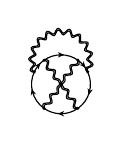
\begin{tikzpicture}[x=0.340cm, y=0.340cm, line width=0.420pt, baseline={([yshift=-0.6ex]0,0)}]
  \draw (-0.631,0.901) arc[start angle=125.000, end angle=55.000, radius=1.100];
  \fill (0.119,1.100) -- (-0.119,1.202) -- (-0.042,1.100) -- (-0.119,0.998) -- cycle;
  \draw (0.631,0.901) arc[start angle=55.000, end angle=25.000, radius=1.100];
  \fill (0.919,0.616) -- (0.844,0.864) -- (0.816,0.739) -- (0.688,0.733) -- cycle;
  \draw (-0.997,0.465) arc[start angle=155.000, end angle=125.000, radius=1.100];
  \fill (-0.766,0.799) -- (-0.998,0.681) -- (-0.870,0.675) -- (-0.841,0.550) -- cycle;
  \draw (0.631,-0.901) arc[start angle=305.000, end angle=235.000, radius=1.100];
  \fill (-0.119,-1.100) -- (0.119,-1.202) -- (0.042,-1.100) -- (0.119,-0.998) -- cycle;
  \draw (0.997,0.465) arc[start angle=25.000, end angle=-55.000, radius=1.100];
  \fill (1.032,-0.400) -- (1.192,-0.196) -- (1.073,-0.244) -- (0.995,-0.143) -- cycle;
  \draw (-0.631,-0.901) arc[start angle=235.000, end angle=155.000, radius=1.100];
  \fill (-1.093,-0.169) -- (-1.130,-0.426) -- (-1.052,-0.325) -- (-0.933,-0.374) -- cycle;
  \draw plot[smooth, tension=0.7] coordinates {(0.657,0.883) (0.679,0.800) (0.669,0.740) (0.616,0.710) (0.531,0.702) (0.446,0.695) (0.393,0.665) (0.383,0.605) (0.405,0.522) (0.426,0.440) (0.417,0.380) (0.363,0.350) (0.279,0.342) (0.194,0.334) (0.146,0.301) (0.143,0.236) (0.152,0.162) (0.141,0.103) (0.103,0.062) (0.061,0.025) (0.026,-0.018) (-0.008,-0.061) (-0.051,-0.099) (-0.088,-0.140) (-0.100,-0.199) (-0.090,-0.273) (-0.093,-0.337) (-0.142,-0.371) (-0.226,-0.379) (-0.311,-0.387) (-0.364,-0.416) (-0.374,-0.477) (-0.352,-0.559) (-0.331,-0.641) (-0.340,-0.702) (-0.394,-0.731) (-0.479,-0.739) (-0.563,-0.747) (-0.617,-0.777) (-0.626,-0.837) (-0.605,-0.919)};
  \draw plot[smooth, tension=0.7] coordinates {(0.605,0.919) (0.626,0.837) (0.617,0.777) (0.563,0.747) (0.479,0.739) (0.394,0.731) (0.340,0.702) (0.331,0.641) (0.352,0.559) (0.374,0.477) (0.364,0.416) (0.311,0.387) (0.226,0.379) (0.142,0.371) (0.093,0.337) (0.090,0.273) (0.100,0.199) (0.088,0.140) (0.051,0.099) (0.008,0.061) (-0.026,0.018) (-0.061,-0.025) (-0.103,-0.062) (-0.141,-0.103) (-0.152,-0.162) (-0.143,-0.236) (-0.146,-0.301) (-0.194,-0.334) (-0.279,-0.342) (-0.363,-0.350) (-0.417,-0.380) (-0.426,-0.440) (-0.405,-0.522) (-0.383,-0.605) (-0.393,-0.665) (-0.446,-0.695) (-0.531,-0.702) (-0.616,-0.710) (-0.669,-0.740) (-0.679,-0.800) (-0.657,-0.883)};
  \draw plot[smooth, tension=0.7] coordinates {(0.967,0.477) (0.924,0.544) (0.913,0.594) (0.951,0.628) (1.025,0.657) (1.099,0.691) (1.133,0.737) (1.112,0.790) (1.050,0.843) (0.986,0.890) (0.958,0.933) (0.982,0.979) (1.042,1.031) (1.098,1.089) (1.114,1.145) (1.076,1.187) (0.999,1.215) (0.923,1.236) (0.882,1.267) (0.888,1.318) (0.925,1.388) (0.958,1.462) (0.953,1.519) (0.902,1.546) (0.821,1.545) (0.742,1.538) (0.693,1.552) (0.681,1.602) (0.691,1.681) (0.695,1.762) (0.671,1.814) (0.614,1.821) (0.539,1.791) (0.467,1.757) (0.416,1.753) (0.387,1.796) (0.369,1.873) (0.345,1.950) (0.304,1.991) (0.248,1.977) (0.188,1.923) (0.132,1.866) (0.086,1.844) (0.044,1.874) (0.000,1.940) (-0.050,2.004) (-0.102,2.027) (-0.150,1.995) (-0.188,1.923) (-0.219,1.850) (-0.255,1.814) (-0.305,1.827) (-0.369,1.873) (-0.438,1.915) (-0.495,1.919) (-0.528,1.872) (-0.539,1.791) (-0.543,1.712) (-0.563,1.665) (-0.614,1.660) (-0.691,1.681) (-0.771,1.696) (-0.826,1.679) (-0.840,1.624) (-0.821,1.545) (-0.797,1.469) (-0.800,1.418) (-0.846,1.395) (-0.925,1.388) (-1.005,1.374) (-1.051,1.339) (-1.044,1.282) (-0.999,1.215) (-0.950,1.152) (-0.935,1.103) (-0.970,1.066) (-1.042,1.031) (-1.112,0.990) (-1.142,0.942) (-1.116,0.890) (-1.050,0.843) (-0.983,0.802) (-0.951,0.761) (-0.971,0.714) (-1.025,0.657) (-1.076,0.594) (-1.088,0.537) (-1.046,0.498) (-0.967,0.477)};
  \draw plot[smooth, tension=0.7] coordinates {(1.026,0.452) (0.984,0.521) (0.974,0.574) (1.013,0.611) (1.088,0.642) (1.162,0.680) (1.196,0.729) (1.176,0.785) (1.114,0.840) (1.050,0.890) (1.022,0.936) (1.046,0.984) (1.105,1.040) (1.161,1.101) (1.176,1.159) (1.137,1.204) (1.060,1.235) (0.983,1.259) (0.941,1.292) (0.946,1.345) (0.982,1.418) (1.012,1.495) (1.007,1.555) (0.954,1.583) (0.871,1.585) (0.790,1.580) (0.739,1.597) (0.725,1.648) (0.733,1.729) (0.735,1.812) (0.709,1.866) (0.650,1.874) (0.571,1.846) (0.497,1.814) (0.444,1.811) (0.412,1.855) (0.391,1.933) (0.364,2.011) (0.321,2.052) (0.262,2.039) (0.199,1.986) (0.141,1.930) (0.092,1.908) (0.047,1.938) (0.000,2.004) (-0.053,2.068) (-0.108,2.091) (-0.158,2.058) (-0.199,1.986) (-0.233,1.913) (-0.272,1.875) (-0.324,1.888) (-0.391,1.933) (-0.463,1.974) (-0.523,1.976) (-0.559,1.928) (-0.571,1.846) (-0.578,1.766) (-0.601,1.717) (-0.654,1.710) (-0.733,1.729) (-0.815,1.742) (-0.872,1.723) (-0.888,1.666) (-0.871,1.585) (-0.849,1.507) (-0.854,1.453) (-0.901,1.428) (-0.982,1.418) (-1.063,1.402) (-1.109,1.364) (-1.104,1.305) (-1.060,1.235) (-1.012,1.169) (-0.998,1.118) (-1.033,1.078) (-1.105,1.040) (-1.175,0.996) (-1.206,0.945) (-1.180,0.891) (-1.114,0.840) (-1.046,0.796) (-1.014,0.753) (-1.034,0.703) (-1.088,0.642) (-1.138,0.577) (-1.149,0.518) (-1.106,0.476) (-1.026,0.452)};
  \draw plot[smooth, tension=0.7] coordinates {(-0.605,0.919) (-0.520,0.912) (-0.466,0.882) (-0.457,0.821) (-0.479,0.739) (-0.500,0.657) (-0.491,0.596) (-0.437,0.567) (-0.352,0.559) (-0.268,0.551) (-0.214,0.522) (-0.205,0.461) (-0.226,0.379) (-0.248,0.297) (-0.233,0.240) (-0.173,0.215) (-0.100,0.199) (-0.048,0.168) (-0.023,0.118) (-0.003,0.065) (0.026,0.018) (0.055,-0.029) (0.075,-0.082) (0.101,-0.131) (0.152,-0.162) (0.225,-0.178) (0.285,-0.203) (0.300,-0.260) (0.279,-0.342) (0.257,-0.424) (0.267,-0.485) (0.320,-0.514) (0.405,-0.522) (0.489,-0.530) (0.543,-0.560) (0.553,-0.620) (0.531,-0.702) (0.509,-0.785) (0.519,-0.845) (0.572,-0.875) (0.657,-0.883)};
  \draw plot[smooth, tension=0.7] coordinates {(-0.657,0.883) (-0.572,0.875) (-0.519,0.845) (-0.509,0.785) (-0.531,0.702) (-0.553,0.620) (-0.543,0.560) (-0.489,0.530) (-0.405,0.522) (-0.320,0.514) (-0.267,0.485) (-0.257,0.424) (-0.279,0.342) (-0.300,0.260) (-0.285,0.203) (-0.225,0.178) (-0.152,0.162) (-0.101,0.131) (-0.075,0.082) (-0.055,0.029) (-0.026,-0.018) (0.003,-0.065) (0.023,-0.118) (0.048,-0.168) (0.100,-0.199) (0.173,-0.215) (0.233,-0.240) (0.248,-0.297) (0.226,-0.379) (0.205,-0.461) (0.214,-0.522) (0.268,-0.551) (0.352,-0.559) (0.437,-0.567) (0.491,-0.596) (0.500,-0.657) (0.479,-0.739) (0.457,-0.821) (0.466,-0.882) (0.520,-0.912) (0.605,-0.919)};
  \fill (0.631,0.901) circle (0.064);
  \fill (0.997,0.465) circle (0.064);
  \fill (-0.631,0.901) circle (0.064);
  \fill (-0.631,-0.901) circle (0.064);
  \fill (0.631,-0.901) circle (0.064);
  \fill (-0.997,0.465) circle (0.064);
\end{tikzpicture}}
\diagramgap
\mbox{$\displaystyle +\,\frac{1}{2}$\,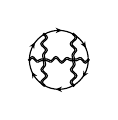
\begin{tikzpicture}[x=0.340cm, y=0.340cm, line width=0.420pt, baseline={([yshift=-0.6ex]0,0)}]
  \draw (-1.100,0.000) arc[start angle=180.000, end angle=120.000, radius=1.100];
  \fill (-0.893,0.653) -- (-1.101,0.498) -- (-0.974,0.514) -- (-0.924,0.396) -- cycle;
  \draw (-0.550,0.953) arc[start angle=120.000, end angle=60.000, radius=1.100];
  \fill (0.119,1.100) -- (-0.119,1.202) -- (-0.042,1.100) -- (-0.119,0.998) -- cycle;
  \draw (-0.550,-0.953) arc[start angle=240.000, end angle=180.000, radius=1.100];
  \fill (-1.012,-0.447) -- (-0.981,-0.704) -- (-0.932,-0.586) -- (-0.805,-0.602) -- cycle;
  \draw (0.550,-0.953) arc[start angle=300.000, end angle=240.000, radius=1.100];
  \fill (-0.119,-1.100) -- (0.119,-1.202) -- (0.042,-1.100) -- (0.119,-0.998) -- cycle;
  \draw (0.550,0.953) arc[start angle=60.000, end angle=0.000, radius=1.100];
  \fill (1.012,0.447) -- (0.981,0.704) -- (0.932,0.586) -- (0.805,0.602) -- cycle;
  \draw (1.100,0.000) arc[start angle=0.000, end angle=-60.000, radius=1.100];
  \fill (0.893,-0.653) -- (1.101,-0.498) -- (0.974,-0.514) -- (0.924,-0.396) -- cycle;
  \draw plot[smooth, tension=0.7] coordinates {(-0.518,0.953) (-0.453,0.893) (-0.426,0.834) (-0.453,0.774) (-0.518,0.714) (-0.583,0.655) (-0.610,0.595) (-0.583,0.536) (-0.518,0.476) (-0.453,0.417) (-0.433,0.357) (-0.468,0.298) (-0.518,0.238) (-0.542,0.179) (-0.535,0.119) (-0.521,0.060) (-0.518,0.000) (-0.515,-0.060) (-0.501,-0.119) (-0.494,-0.179) (-0.518,-0.238) (-0.568,-0.298) (-0.603,-0.357) (-0.583,-0.417) (-0.518,-0.476) (-0.453,-0.536) (-0.426,-0.595) (-0.453,-0.655) (-0.518,-0.714) (-0.583,-0.774) (-0.610,-0.834) (-0.583,-0.893) (-0.518,-0.953)};
  \draw plot[smooth, tension=0.7] coordinates {(-0.582,0.953) (-0.517,0.893) (-0.490,0.834) (-0.517,0.774) (-0.582,0.714) (-0.647,0.655) (-0.674,0.595) (-0.647,0.536) (-0.582,0.476) (-0.517,0.417) (-0.497,0.357) (-0.532,0.298) (-0.582,0.238) (-0.606,0.179) (-0.599,0.119) (-0.585,0.060) (-0.582,0.000) (-0.579,-0.060) (-0.565,-0.119) (-0.558,-0.179) (-0.582,-0.238) (-0.632,-0.298) (-0.667,-0.357) (-0.647,-0.417) (-0.582,-0.476) (-0.517,-0.536) (-0.490,-0.595) (-0.517,-0.655) (-0.582,-0.714) (-0.647,-0.774) (-0.674,-0.834) (-0.647,-0.893) (-0.582,-0.953)};
  \draw plot[smooth, tension=0.7] coordinates {(0.582,0.953) (0.647,0.893) (0.674,0.834) (0.647,0.774) (0.582,0.714) (0.517,0.655) (0.490,0.595) (0.517,0.536) (0.582,0.476) (0.647,0.417) (0.667,0.357) (0.632,0.298) (0.582,0.238) (0.558,0.179) (0.565,0.119) (0.579,0.060) (0.582,0.000) (0.585,-0.060) (0.599,-0.119) (0.606,-0.179) (0.582,-0.238) (0.532,-0.298) (0.497,-0.357) (0.517,-0.417) (0.582,-0.476) (0.647,-0.536) (0.674,-0.595) (0.647,-0.655) (0.582,-0.714) (0.517,-0.774) (0.490,-0.834) (0.517,-0.893) (0.582,-0.953)};
  \draw plot[smooth, tension=0.7] coordinates {(0.518,0.953) (0.583,0.893) (0.610,0.834) (0.583,0.774) (0.518,0.714) (0.453,0.655) (0.426,0.595) (0.453,0.536) (0.518,0.476) (0.583,0.417) (0.603,0.357) (0.568,0.298) (0.518,0.238) (0.494,0.179) (0.501,0.119) (0.515,0.060) (0.518,0.000) (0.521,-0.060) (0.535,-0.119) (0.542,-0.179) (0.518,-0.238) (0.468,-0.298) (0.433,-0.357) (0.453,-0.417) (0.518,-0.476) (0.583,-0.536) (0.610,-0.595) (0.583,-0.655) (0.518,-0.714) (0.453,-0.774) (0.426,-0.834) (0.453,-0.893) (0.518,-0.953)};
  \draw plot[smooth, tension=0.7] coordinates {(-1.100,0.032) (-1.045,0.097) (-0.990,0.124) (-0.935,0.097) (-0.880,0.032) (-0.825,-0.018) (-0.770,-0.021) (-0.715,0.008) (-0.660,0.032) (-0.605,0.035) (-0.550,0.032) (-0.495,0.035) (-0.440,0.032) (-0.385,0.008) (-0.330,-0.021) (-0.275,-0.018) (-0.220,0.032) (-0.165,0.097) (-0.110,0.124) (-0.055,0.097) (0.000,0.032) (0.055,-0.033) (0.110,-0.060) (0.165,-0.033) (0.220,0.032) (0.275,0.082) (0.330,0.085) (0.385,0.056) (0.440,0.032) (0.495,0.029) (0.550,0.032) (0.605,0.029) (0.660,0.032) (0.715,0.056) (0.770,0.085) (0.825,0.082) (0.880,0.032) (0.935,-0.033) (0.990,-0.060) (1.045,-0.033) (1.100,0.032)};
  \draw plot[smooth, tension=0.7] coordinates {(-1.100,-0.032) (-1.045,0.033) (-0.990,0.060) (-0.935,0.033) (-0.880,-0.032) (-0.825,-0.082) (-0.770,-0.085) (-0.715,-0.056) (-0.660,-0.032) (-0.605,-0.029) (-0.550,-0.032) (-0.495,-0.029) (-0.440,-0.032) (-0.385,-0.056) (-0.330,-0.085) (-0.275,-0.082) (-0.220,-0.032) (-0.165,0.033) (-0.110,0.060) (-0.055,0.033) (0.000,-0.032) (0.055,-0.097) (0.110,-0.124) (0.165,-0.097) (0.220,-0.032) (0.275,0.018) (0.330,0.021) (0.385,-0.008) (0.440,-0.032) (0.495,-0.035) (0.550,-0.032) (0.605,-0.035) (0.660,-0.032) (0.715,-0.008) (0.770,0.021) (0.825,0.018) (0.880,-0.032) (0.935,-0.097) (0.990,-0.124) (1.045,-0.097) (1.100,-0.032)};
  \fill (-0.550,0.953) circle (0.064);
  \fill (0.550,0.953) circle (0.064);
  \fill (-1.100,0.000) circle (0.064);
  \fill (-0.550,-0.953) circle (0.064);
  \fill (1.100,0.000) circle (0.064);
  \fill (0.550,-0.953) circle (0.064);
\end{tikzpicture}}
\diagramgap
\mbox{$\displaystyle -\,\frac{1}{6}$\,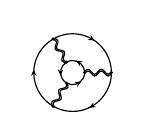
\begin{tikzpicture}[x=0.340cm, y=0.340cm, line width=0.420pt, baseline={([yshift=-0.6ex]0,0)}]
  \draw (-0.725,1.256) arc[start angle=120.000, end angle=0.000, radius=1.450];
  \fill (0.828,1.196) -- (0.673,1.404) -- (0.689,1.277) -- (0.571,1.227) -- cycle;
  \draw (1.450,0.000) arc[start angle=360.000, end angle=240.000, radius=1.450];
  \fill (0.622,-1.315) -- (0.879,-1.284) -- (0.761,-1.235) -- (0.777,-1.108) -- cycle;
  \draw (-0.725,-1.256) arc[start angle=240.000, end angle=120.000, radius=1.450];
  \fill (-1.450,0.119) -- (-1.552,-0.119) -- (-1.450,-0.042) -- (-1.348,-0.119) -- cycle;
  \draw (-0.225,-0.390) arc[start angle=240.000, end angle=360.000, radius=0.450];
  \fill (0.328,-0.330) -- (0.071,-0.361) -- (0.189,-0.411) -- (0.173,-0.538) -- cycle;
  \draw (0.450,0.000) arc[start angle=0.000, end angle=120.000, radius=0.450];
  \fill (0.122,0.449) -- (0.277,0.242) -- (0.261,0.369) -- (0.379,0.418) -- cycle;
  \draw (-0.225,0.390) arc[start angle=120.000, end angle=240.000, radius=0.450];
  \fill (-0.450,-0.119) -- (-0.348,0.119) -- (-0.450,0.042) -- (-0.552,0.119) -- cycle;
  \draw plot[smooth, tension=0.7] coordinates {(1.450,-0.032) (1.388,-0.097) (1.325,-0.124) (1.262,-0.097) (1.200,-0.032) (1.138,0.033) (1.075,0.060) (1.012,0.033) (0.950,-0.032) (0.888,-0.097) (0.825,-0.124) (0.762,-0.097) (0.700,-0.032) (0.638,0.033) (0.575,0.060) (0.512,0.033) (0.450,-0.032)};
  \draw plot[smooth, tension=0.7] coordinates {(1.450,0.032) (1.388,-0.033) (1.325,-0.060) (1.262,-0.033) (1.200,0.032) (1.138,0.097) (1.075,0.124) (1.012,0.097) (0.950,0.032) (0.888,-0.033) (0.825,-0.060) (0.762,-0.033) (0.700,0.032) (0.638,0.097) (0.575,0.124) (0.512,0.097) (0.450,0.032)};
  \draw plot[smooth, tension=0.7] coordinates {(-0.753,-1.240) (-0.778,-1.153) (-0.770,-1.086) (-0.715,-1.045) (-0.628,-1.023) (-0.540,-1.002) (-0.486,-0.961) (-0.478,-0.893) (-0.503,-0.807) (-0.528,-0.720) (-0.520,-0.653) (-0.465,-0.612) (-0.378,-0.590) (-0.290,-0.569) (-0.236,-0.528) (-0.228,-0.460) (-0.253,-0.374)};
  \draw plot[smooth, tension=0.7] coordinates {(-0.697,-1.272) (-0.722,-1.185) (-0.714,-1.118) (-0.660,-1.077) (-0.572,-1.055) (-0.485,-1.034) (-0.430,-0.993) (-0.422,-0.925) (-0.447,-0.839) (-0.472,-0.752) (-0.464,-0.685) (-0.410,-0.644) (-0.322,-0.622) (-0.235,-0.601) (-0.180,-0.560) (-0.172,-0.492) (-0.197,-0.406)};
  \draw plot[smooth, tension=0.7] coordinates {(-0.697,1.272) (-0.610,1.250) (-0.555,1.209) (-0.547,1.142) (-0.572,1.055) (-0.597,0.969) (-0.589,0.901) (-0.535,0.860) (-0.447,0.839) (-0.360,0.817) (-0.305,0.776) (-0.297,0.709) (-0.322,0.622) (-0.347,0.536) (-0.339,0.468) (-0.285,0.427) (-0.197,0.406)};
  \draw plot[smooth, tension=0.7] coordinates {(-0.753,1.240) (-0.665,1.218) (-0.611,1.177) (-0.603,1.110) (-0.628,1.023) (-0.653,0.937) (-0.645,0.869) (-0.590,0.828) (-0.503,0.807) (-0.415,0.785) (-0.361,0.744) (-0.353,0.677) (-0.378,0.590) (-0.403,0.504) (-0.395,0.436) (-0.340,0.395) (-0.253,0.374)};
  \fill (1.450,0.000) circle (0.064);
  \fill (-0.725,-1.256) circle (0.064);
  \fill (-0.725,1.256) circle (0.064);
  \fill (0.450,0.000) circle (0.064);
  \fill (-0.225,0.390) circle (0.064);
  \fill (-0.225,-0.390) circle (0.064);
\end{tikzpicture}}
\diagramgap
\mbox{$\displaystyle -\,\frac{1}{6}$\,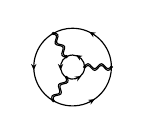
\begin{tikzpicture}[x=0.340cm, y=0.340cm, line width=0.420pt, baseline={([yshift=-0.6ex]0,0)}]
  \draw (-0.725,-1.256) arc[start angle=240.000, end angle=360.000, radius=1.450];
  \fill (0.828,-1.196) -- (0.571,-1.227) -- (0.689,-1.277) -- (0.673,-1.404) -- cycle;
  \draw (1.450,0.000) arc[start angle=0.000, end angle=120.000, radius=1.450];
  \fill (0.622,1.315) -- (0.777,1.108) -- (0.761,1.235) -- (0.879,1.284) -- cycle;
  \draw (-0.725,1.256) arc[start angle=120.000, end angle=240.000, radius=1.450];
  \fill (-1.450,-0.119) -- (-1.348,0.119) -- (-1.450,0.042) -- (-1.552,0.119) -- cycle;
  \draw (-0.225,-0.390) arc[start angle=240.000, end angle=360.000, radius=0.450];
  \fill (0.328,-0.330) -- (0.071,-0.361) -- (0.189,-0.411) -- (0.173,-0.538) -- cycle;
  \draw (0.450,0.000) arc[start angle=0.000, end angle=120.000, radius=0.450];
  \fill (0.122,0.449) -- (0.277,0.242) -- (0.261,0.369) -- (0.379,0.418) -- cycle;
  \draw (-0.225,0.390) arc[start angle=120.000, end angle=240.000, radius=0.450];
  \fill (-0.450,-0.119) -- (-0.348,0.119) -- (-0.450,0.042) -- (-0.552,0.119) -- cycle;
  \draw plot[smooth, tension=0.7] coordinates {(1.450,-0.032) (1.388,-0.097) (1.325,-0.124) (1.262,-0.097) (1.200,-0.032) (1.138,0.033) (1.075,0.060) (1.012,0.033) (0.950,-0.032) (0.888,-0.097) (0.825,-0.124) (0.762,-0.097) (0.700,-0.032) (0.638,0.033) (0.575,0.060) (0.512,0.033) (0.450,-0.032)};
  \draw plot[smooth, tension=0.7] coordinates {(1.450,0.032) (1.388,-0.033) (1.325,-0.060) (1.262,-0.033) (1.200,0.032) (1.138,0.097) (1.075,0.124) (1.012,0.097) (0.950,0.032) (0.888,-0.033) (0.825,-0.060) (0.762,-0.033) (0.700,0.032) (0.638,0.097) (0.575,0.124) (0.512,0.097) (0.450,0.032)};
  \draw plot[smooth, tension=0.7] coordinates {(-0.697,1.272) (-0.610,1.250) (-0.555,1.209) (-0.547,1.142) (-0.572,1.055) (-0.597,0.969) (-0.589,0.901) (-0.535,0.860) (-0.447,0.839) (-0.360,0.817) (-0.305,0.776) (-0.297,0.709) (-0.322,0.622) (-0.347,0.536) (-0.339,0.468) (-0.285,0.427) (-0.197,0.406)};
  \draw plot[smooth, tension=0.7] coordinates {(-0.753,1.240) (-0.665,1.218) (-0.611,1.177) (-0.603,1.110) (-0.628,1.023) (-0.653,0.937) (-0.645,0.869) (-0.590,0.828) (-0.503,0.807) (-0.415,0.785) (-0.361,0.744) (-0.353,0.677) (-0.378,0.590) (-0.403,0.504) (-0.395,0.436) (-0.340,0.395) (-0.253,0.374)};
  \draw plot[smooth, tension=0.7] coordinates {(-0.753,-1.240) (-0.778,-1.153) (-0.770,-1.086) (-0.715,-1.045) (-0.628,-1.023) (-0.540,-1.002) (-0.486,-0.961) (-0.478,-0.893) (-0.503,-0.807) (-0.528,-0.720) (-0.520,-0.653) (-0.465,-0.612) (-0.378,-0.590) (-0.290,-0.569) (-0.236,-0.528) (-0.228,-0.460) (-0.253,-0.374)};
  \draw plot[smooth, tension=0.7] coordinates {(-0.697,-1.272) (-0.722,-1.185) (-0.714,-1.118) (-0.660,-1.077) (-0.572,-1.055) (-0.485,-1.034) (-0.430,-0.993) (-0.422,-0.925) (-0.447,-0.839) (-0.472,-0.752) (-0.464,-0.685) (-0.410,-0.644) (-0.322,-0.622) (-0.235,-0.601) (-0.180,-0.560) (-0.172,-0.492) (-0.197,-0.406)};
  \fill (1.450,0.000) circle (0.064);
  \fill (-0.725,1.256) circle (0.064);
  \fill (-0.725,-1.256) circle (0.064);
  \fill (0.450,0.000) circle (0.064);
  \fill (-0.225,0.390) circle (0.064);
  \fill (-0.225,-0.390) circle (0.064);
\end{tikzpicture}}
